%%%%%%%%Bilecik Şeyh Edebali Üniversitesi Mühendsilik Fakültesi%%%% 
%%%%%%%%Bilgisayar Mühendisliği Bitirme Çalışması%%%%%%%%%%%%%%%%%%
%%%%%%%%%%%%%%%%%%%%%%LaTeX Class%%%%%%%%%%%%%%%%%%%%%%%%%%%%%%%%%%
\documentclass{BUB}
\addbibresource{references.bib}
%%%%%%%%%%%%%%%%%%%%%%%%%%%%%%%%%%%%%%%%%%%%%%%%%%%%%%%%%%%%%%%%%%%
\begin{document}
%%%%%%%%%%%%%%%%%%%%%%Bitirme Çalışmasının Bölümleri%%%%%%%%%%%%%%% 
\thispagestyle{empty}
\begin{figure}[H]
\centering

\includegraphics[scale=0.2]{logomuz}
\end{figure}

\begin{center}
\textbf{T.C.}\\
\textbf{BİLECİK ŞEYH EDEBALİ ÜNİVERSİTESİ}\\
\textbf{MÜHENDİSLİK FAKÜLTESİ}

\textbf{BİLGİSAYAR MÜHENDİSLİĞİ BÖLÜMÜ}
\end{center}
\vfill
\begin{center}
\textbf{Docker ile çoklu konteynerlar kullanarak paralel iş yapan sistem tasarımı }

\textbf{Aleyna ÇELİK \\ IBRAHIM KHALIL ATTEIB YACOUB}

\textbf{BİTİRME ÇALIŞMASI}
\end{center}
\vfill
\begin{center}
\textbf{DANIŞMANI : Prof. Dr. Cihan KARAKUZU \\ Dr. Öğr. Üyesi Burakhan ÇUBUKÇU}

\textbf{BİLECİK}\\ 
\textbf{\today}
\end{center}


\thispagestyle{empty}
\begin{figure}[H]
\centering

\includegraphics[scale=0.2]{logomuz}
\end{figure}

\begin{center}
\textbf{T.C.}\\
\textbf{BİLECİK ŞEYH EDEBALİ ÜNİVERSİTESİ}\\
\textbf{MÜHENDİSLİK FAKÜLTESİ}

\textbf{BİLGİSAYAR MÜHENDİSLİĞİ BÖLÜMÜ}
\end{center}
\vfill
\begin{center}
\textbf{Web Tabanlı Konteyner Orkestrasyon Sistemi }

\textbf{ALEYNA ÇELİK \\ IBRAHIM KHALIL ATTEIB YACOUB}

\textbf{BİTİRME ÇALIŞMASI}
\end{center}
\vfill
\begin{center}
\textbf{DANIŞMANI :\\ Prof. Dr. Cihan KARAKUZU \\ Dr. Öğr. Üyesi Burakhan ÇUBUKÇU}

\textbf{BİLECİK}\\ 
\textbf{\today}
\end{center}


\pagenumbering{roman} % romen rakamları kullanılmaya başlanıyor.
\setcounter{page}{2}  % sayfa numarasını ii'den başlatılıyor.
\begin{center}
\textbf{BİLDİRİM}
\end{center}
\begin{singlespace}%1 satır aralığı
Bu çalışmada bütün bilgilerin etik davranış ve akademik kurallar çerçevesinde elde edildiğini ve yazım kurallarına uygun olarak hazırlanan bu çalışmada bana ait olmayan her türlü ifade ve bilginin kaynağına eksiksiz atıf yapıldığını bildiririm.
\end{singlespace}
\vspace{2cm}

\begin{center}
\textbf{DECLARATION}
\end{center}
\begin{singlespace}
I hereby declare that all information in this document has been obtained and presented in accordance with academic rules and ethical conduct. I also declare that, as required by these rules and conduct, I have fully cited and referenced all materials and results that are not original to this work.
\end{singlespace}

\vspace{3cm}
\begin{flushright}
\begin{minipage}{5cm}
\begin{center}
\textbf{İmza}

\textbf{ALEYNA ÇELİK \\ IBRAHIM KHALIL ATTEIB YACOUB}

\textbf{Tarih: {\today}}\hfill
\end{center}
\end{minipage}
\end{flushright}

\begin{center}
{\bf{\large ÖZET}\vspace*{.5cm}

BİTİRME ÇALIŞMASI

Docker ile çoklu konteynerlar kullanarak paralel iş yapan sistem tasarımı

Aleyna ÇELİK \\ Ibrahim Khalil Atteib YACOUB}

\begin{singlespace}
{\bfseries
Bilecik Şeyh Edebali Üniversitesi\\
Mühendislik Fakültesi\\
Bilgisayar Mühendisliği Bölümü}
\end{singlespace}

{\bf Danışman: Prof. Dr. Cihan KARAKUZU \\ Dr. Öğr. Üyesi Burakhan ÇUBUKÇU}

{\bf \the\year, \ref{TotPages} Sayfa}

\begin{tabular}{p{7cm}p{2cm}p{4cm}}
\center\textbf{Jüri\; Üyeleri}&&\center\textbf{İmza}\cr
\dotfill&&\dotfill\\
\dotfill&&\dotfill\\
\dotfill&&\dotfill
\end{tabular}
\end{center}
{\small  Docker ile çoklu konteynerlar kullanarak paralel işlem yapan sistemler, uygulama ve servislerin farklı konteynerlar içinde izole edilerek çalıştırılmasını sağlayan bir sistem tasarımıdır. Bu sayede her bir konteyner, farklı özellikler ve işlevler için optimize edilebilir ve uygulama ölçeklenebilir hale gelir.
Ayrıca, verilen işi  belirtilen sayıda konteyner ile bölerek daha esnek hale getirmek amaçlanmıştır. Arayüz, canlı olarak ekranda ilerleme bilgileri göstererek, kullanıcılara toplam iş miktarı ile tamamlanma yüzdesi ve hangi konteynerların en hızlı olduğu gibi önemli bilgileri verir.
Bu arayüz, güvenlik testleri veya izinsiz giriş girişimi gibi meşru olmayan amaçlarla kullanılmamalıdır.}


%%%%%%%%%%%%%%%%%%%%%%%%%%%%%%%%%%%%%%%%%%%%%%%%%%%%%%%%%%%%%%%%%%% 
\newpage
\begin{center}
{\bf{\large ABSTRACT}\vspace*{.5cm}

THESIS

System design using Docker with multiple containers for parallel processing

Aleyna ÇELİK \\ IBRAHIM KHALIL ATTEIB YACOUB}

\begin{singlespace}
{\bf
Bilecik Şeyh Edebali University\\
Engineering Faculty\\
Department of Computer Engineering}
\end{singlespace}

{\bf Advisor : Prof. Dr. Cihan KARAKUZU \\ Assoc. Prof. Dr. Burakhan ÇUBUKÇU

\the\year, \ref{TotPages} Pages}

\begin{tabular}{p{7cm}p{2cm}p{4cm}}
\center \textbf{Jury}&&\center \textbf{Sign}\cr
\dotfill& &\dotfill\\
\dotfill& &\dotfill\\
\dotfill& &\dotfill
\end{tabular}
\end{center}
{\small Using multiple containers with Docker to perform parallel processing is a system design that allows applications and services to be run in different containers, isolated from each other. This allows each container to be optimized for different features and functions, making the application scalable. Additionally, the system is designed to make the given task more flexible by dividing it into a specified number of containers. The interface displays progress information live on the screen, providing users with important information such as the total amount of work completed, the completion percentage, and which containers are the fastest. However, this interface should not be used for illegitimate purposes such as security testing or unauthorized access attempts. }



\addcontentsline{toc}{section}{ÖNSÖZ}
\section*{ÖNSÖZ}
Bitirme çalışmasında başından sonuna kadar emeği geçen ve bizi bu konuya yönlendiren saygı değer hocalarımız ve danışmanlarımız Sayın Prof. Dr. Cihan KARAKUZU ve Dr. Öğr. Üyesi Burakhan ÇUBUKÇU'a tüm katkılarından ve hiç eksiltmediği desteklerinden dolayı teşekkür ederiz.

\begin{flushright}
\textbf{Aleyna ÇELİK \\ Ibrahim Khalil Atteib YACOUB}

\today
\end{flushright}
%%%İçindekiler ve tablolar%%%%%%%%%%%%%%
%%%%%%%%%%%%%%%%%%%%%%İÇİNDEKİLER%%%%%%%%%%%%%
\tableofcontents
%%%%%%%%%%%%%%%%ŞEKİLLER TABLOSU%%%%%%%%%%%%%%
\renewcommand*\listfigurename{\centerline{\normalsize ŞEKİLLER TABLOSU}}
\listoffigures%bu komutun olduğu yerde şekiller listesi oluşturulur
\addcontentsline{toc}{section}{\normalsize ŞEKİLLER TABLOSU}
%%%%%%%%%%%%%%%%%%%%%%ÇİZELGELER TABLOSU%%%%%%%%%%%%%%%%%
\renewcommand*\listtablename{\centerline{\normalsize ÇİZELGELER TABLOSU}}
\listoftables%bu komutun olduğu yerde tablolar listesi oluşturulur
\addcontentsline{toc}{section}{ÇİZELGELER TABLOSU}
%%%%%%%%%%%%%%%%%%%%%ÇİZELGELER TABLOSU%%%%%%%%%%%%%%%%%
%\textbf{\centerline{SİMGELER VE KISALTMALAR}}
\addcontentsline{toc}{section}{SİMGELER VE KISALTMALAR}


\pagenumbering{arabic}  % Sayfa numaralamasını arap rakamlarıyla yapar.
\setcounter{page}{1}    % sayfa numarasını 1'den başlatır.
\section{GİRİŞ}
Günümüzde teknolojik projelerin karmaşıklığı ve iş yükünün artmasıyla birlikte, verimli ve ölçeklenebilir bir altyapı tasarımı büyük önem taşımaktadır. Bu nedenle, Web Tabanlı Konteyner Orkestrasyon Sistemi, proje olarak ideal bir çözüm değerlendirilmiştir.

Konteyner kavramı, ilk olarak 1979 yılında ortaya atılmış ve o tarihten itibaren gelişimini sürdürmüştür. Bu süreçte Unix V7 ile ilk kez kullanılmıştır. FreeBSD Jails, Linux VServer, Oracle Solaris Containers, Open VZ, Process Containers (Google), LXC, Warden ve Lmctfy gibi gelişim süreçlerinden geçerek günümüze kadar gelmiştir.

Konteyner teknolojisinin daha yaygın hale gelmesi, 2000'li yılların başında FreeBSD Jail ile gerçekleşmiştir. Ardından Jacques Gélinas'in VServer projesi ile Linux ortamına dahil olmuştur. Bu temel altyapının oluşturulmasının ardından, günümüz Linux konteynerlerinin yapısı şekillenmeye başlamıştır.

Ancak, konteyner teknolojisi bu gelişmelere rağmen hala genel kullanım için yaygın değildi. 2008 yılında Docker, bu alanda devrim niteliğinde bir adım atmıştır. Google gibi büyük bilgi teknolojileri şirketlerinin kullandığı bu sistem, son kullanıcıların da hizmetine sunulmuş ve konteyner teknolojisinin hızla gelişmesine yol açmıştır. Docker, kendi adını taşıyan konteyner teknolojisiyle (dotCloud aracılığıyla) kullanıcıları tanıştırmıştır.\cite{container}

Bu proje için Docker'ın kullanılması uygun görülmüştür. Bunun temel nedenleri arasında hafiflik, taşınabilirlik, ölçeklenebilirlik, kolay dağıtım ve yönetim, izolasyon ve güvenlik avantajları bulunmaktadır. Bu tasarım yaklaşımı, projenin gereksinimlerini etkin bir şekilde karşılamak ve iş yükünü yönetmek için ideal bir çözüm sunmaktadır.

Projeyle ilgili yapılan araştırmanın bir bölümü olan Literatür Taraması, sonraki bölümde detaylı olarak açıklanmıştır.
\section{Literatür Taraması}
Konteynerizasyon konusunda akademik çalışmalar 2008 yıllarında başlamış, 2013 yıllarından sonra yoğunlaşmıştır. Bu projede konuya yakın olan daha önce yapılan çalışmalar aşağıda özetlenmiştir.

"An Overview of Containerization Technology: Advantages, Challenges, and Future Directions" adlı çalışmada, yazarlar containerization teknolojisinin genel bir bakışını, avantajlarını, zorluklarını ve gelecekteki yönelimlerini ele almaktadır. Makale, containerization teknolojisinin nasıl çalıştığına, sanallaştırma teknolojileriyle karşılaştırılmasına ve çeşitli kullanım senaryolarına odaklanmaktadır \cite{Smith_Emily}.

"Docker for Multi-containers Web Application" başlıklı makalede, Sharma, Saxena ve Singh, çoklu konteyner web uygulamaları için Docker teknolojisini ele almaktadır. Makale, 2020 2. Uluslararası Sanayi Uygulamaları İçin Yenilikçi Mekanizmalar Konferansı'nda sunulmuştur. Yazarlar, Docker teknolojisinin kullanımıyla çoklu konteyner web uygulamalarının nasıl hazırlanacağını ve dağıtılacağını ele almaktadırlar. Makalede, Docker'in kullanımının avantajları ve web uygulamaları için uygunluğu da tartışılmaktadır \cite{sharma2020docker}.

"Containerization: A Systematic Literature Review" başlıklı çalışma, containerization teknolojisi hakkında sistematik bir literatür taraması sunmaktadır. Yazarlar, containerization teknolojisinin farklı yönlerini, kullanım alanlarını, avantajlarını ve zorluklarını analiz etmektedirler. Ayrıca, çalışmada gelecekteki araştırma yönelimleri ve containerization teknolojisinin geliştirilmesi için öneriler de sunulmaktadır.\cite{Brown_Jennifer}

"Mastering Docker" adlı kitap, Docker teknolojisi hakkında kapsamlı bir kılavuz sunmaktadır. Okuyucular, Docker'ın nasıl kullanılacağı, konteynerlerin nasıl tasarlanacağı, dağıtılacağı ve yönetileceği hakkında bilgi edinebilirler. Kitap, uygulama geliştirme ve dağıtım süreçlerinde Docker'ın nasıl kullanılabileceği konusunda pratik bilgiler sunmaktadır. Sonuç olarak, "Mastering Docker" kitabı, Docker teknolojisi hakkında kapsamlı bir kılavuz sunarak, okuyucuların konteynerleştirme ve DevOps becerilerini geliştirmelerine yardımcı olmayı amaçlamaktadır \cite{mckendrick2020mastering}.

"On Enhancing the Orchestration of Multi-container Docker Applications" başlıklı makale, Docker teknolojisi ile oluşturulmuş çoklu konteynerli uygulamaların orkestrasyonunu geliştirmek için Docker Compose ile bir alternatif yaklaşım sunmaktadır. Bu çalışma, yazılım geliştiricilere ve sistem yöneticilerine fayda sağlamayı amaçlamaktadır \cite{brogi2020enhancing}.

"Docker Compose'un Çok Bileşenli Sistemleri Oluşturmak İçin Kullanımının İncelenmesi" başlıklı makale, Docker Compose'un kullanımının çoğu zaman çok bileşenli sistemlerin oluşturulması için yararlı olduğunu inceliyor. Bununla birlikte, Docker Compose dosyalarının kullanımı konusunda belirli zorluklar da bulunmaktadır. Örneğin, Docker Compose dosyalarının oluşturulması ve yönetilmesi karmaşık olabilir ve Docker Compose dosyalarının sürdürülebilirliği sorunları ortaya çıkabilir \cite{ibrahim2021study}.

Bu literatür taraması, Docker teknolojisi ve konteynerleştirme üzerine yapılmış bazı çalışmaları özetlemektedir. Bu çalışmalar, Docker'ın çoklu konteyner uygulamaları, orkestrasyon yöntemleri ve kullanım zorlukları gibi farklı yönlerini ele almaktadır. Bu bilgiler, bu projede kullanılan teknolojik seçimlerin nedenleri ve özellikleri hakkında bilgi vermektedir.
\section{KULLANILAN TEKNOLOJİLER}
Bu çalışmada kullanılan teknolojilerin tercih sebepleri ve özellikleri detaylıca aşağıda bahsedilmiştir.
\subsection{Docker}\label{subsec:docker}
Docker, yazılım uygulamalarını konteynerlere paketleme ve dağıtma konusunda kullanılan bir platformdur. Bu teknoloji, uygulamaların bağımsız bir şekilde çalışabilmesini sağlar ve kurulum ve dağıtım süreçlerini kolaylaştırır. Docker, bir uygulamanın çalışması için gerekli olan tüm bağımlılıkları içeren bir konteyner oluşturmanızı sağlar. Bu konteyner, farklı ortamlarda (geliştirme, test, üretim) aynı şekilde çalışabilir, uyumluluk sorunlarını en aza indirir ve uygulamaların taşınabilirliğini artırır. Docker, yüksek verimlilik ve izolasyon sağlar, kaynakların daha etkili kullanılmasını sağlar ve sistem yönetimini kolaylaştırır \cite{docker}.\\
Bu çalışmada kullanılan Docker özellikleri:
\begin{itemize}
  \item \textbf{Docker compose}: Docker ortamında birden fazla konteyneri yönetmek için kullanılan bir araçtır. Docker Compose, bir YAML dosyası aracılığıyla konteynerleri tanımlamanıza ve yapılandırmanıza olanak sağlar. Bu YAML dosyasında, farklı konteynerlerin konfigürasyonları, ağ bağlantıları, bağımlılıkları ve diğer özellikleri belirtilebilir. Docker Compose, bu dosyayı okuyarak ve yorumlayarak belirtilen konteynerleri oluşturur, başlatır ve durdurur. Böylece birden fazla konteynerin aynı ortamda birlikte çalışmasını kolaylaştırır.
  \item \textbf{Docker Engine API}: Docker ortamını yönetmek için kullanılan bir programlama arabirimidir. Docker Engine, Docker'ın temel bileşenidir ve konteynerlerin oluşturulması, çalıştırılması ve yönetilmesi gibi işlemleri gerçekleştirir. Docker Engine API, Docker ortamının komut satırı arayüzünün (CLI) ötesine geçerek programatik olarak Docker ortamını kontrol etmenizi sağlar. Bu API, Docker ile etkileşim kurmanızı ve Docker işlemlerini otomatikleştirmenizi sağlayan bir dizi yöntem ve işlev sağlar. Docker Engine API, HTTP üzerinden erişilebilen bir RESTful API olarak sunulur ve Docker komutlarını programlamaya entegre etmenize olanak tanır \cite{docker_api_reference}.
\end{itemize}

\subsection{Laravel}
Laravel, PHP tabanlı bir web uygulama geliştirme framework'üdür. MVC (Model-View-Controller) tasarım desenini benimser ve geliştiricilere web uygulamaları oluşturmak için bir dizi kullanışlı özellik sunar. Laravel, güçlü bir yönlendirme sistemi, otomatik olarak oluşturulan SQL sorguları, oturum yönetimi, veritabanı migrasyonları, önbellekleme, form doğrulama gibi birçok bileşeni içerir. Bu bileşenler, geliştirme sürecini hızlandırır ve kod tekrarını azaltır. Laravel'in geniş bir topluluğu vardır ve bu da destek almak ve kaynaklara erişmek açısından avantaj sağlar \cite{laravel_documentation}.\\
Bu çalışmada kullanılan Laravel özelliklerine kısaca bir göz atalım:
\begin{itemize}
  \item \textbf{Migration (migrasyon)} : Laravel, veritabanı tablolarını oluşturmak ve yönetmek için migrasyonları kullanır. Migrasyonlar, veritabanı şemalarını kod olarak temsil eder ve veritabanı yapısının kolayca değiştirilmesini ve sürdürülmesini sağlar.
  \item \textbf{Model} : Laravel'de model, veritabanı tablolarıyla ilişkilendirilen veri erişim katmanını temsil eder. Model sınıfları, veritabanı işlemlerini gerçekleştirmek ve verileri işlemek için kullanılır.
  \item \textbf{Request} :  Laravel, HTTP isteklerini işlemek için request (istek) sınıflarını kullanır. Bu sınıflar, gelen istek verilerini doğrulamak, işlemek ve manipüle etmek için kullanılır.
  \item \textbf{Controller} : Laravel'de controller (denetleyici), HTTP isteklerini yöneten ve ilgili iş mantığını uygulayan sınıflardır. Bir controller, bir veya daha fazla işlem (action) içerir ve bu işlemler, isteklere yanıt olarak çalıştırılır.
  \item \textbf{Route} : Laravel, yönlendirme (routing) mekanizmasıyla istekleri doğru controller ve işlemle eşleştirir. Route dosyalarında, URL'leri belirleyebilir, istek yönlendirmelerini tanımlayabilir ve parametreleri yakalayabilirsiniz.
  \item \textbf{Queue} : Laravel, işleri (jobs) arkaplanda sıralı olarak çalıştırmak için kuyruk (queue) sistemini destekler. Kuyruklar, yoğun işlem yükü altında olan uygulamalarda işleri geciktirir ve daha sonra işlerin işlenmesini sağlar.
  \item \textbf{Auth} : Laravel'in sağladığı kimlik doğrulama (authentication) sistemi. Auth bileşeni, kullanıcı kaydı, oturum yönetimi, şifre sıfırlama gibi kullanıcı kimlik doğrulama işlemlerini kolaylaştırır.
  \item \textbf{Event/Listener} : Laravel'de "Event" ve "Listener" kavramları, olay tabanlı programlama yaklaşımını desteklemek için kullanılır. Bir "Event" (olay), uygulamanızda gerçekleşen belirli bir eylemi veya durumu temsil eder.
  \item \textbf{View} : Laravel'de "View" (görünüm), kullanıcılara sunulan HTML veya JSON gibi çıktıları oluşturmak için kullanılan şablon dosyalarını temsil eder. Görünümler, uygulama mantığını içermeyen, yalnızca kullanıcı arayüzünü temsil eden yapıları içerir.
\end{itemize}
\subsection{MySQL}
MySQL, popüler bir açık kaynaklı ilişkisel veritabanı yönetim sistemidir. MySQL, verilerin depolanması, yönetilmesi ve erişilmesi için kullanılır. Ölçeklenebilir, güvenilir ve performanslı bir veritabanı sunucusu olarak bilinir. MySQL, geniş bir kullanıcı tabanına ve gelişmiş özelliklere sahiptir. SQL (Structured Query Language) tabanlı bir veritabanı yönetim sistemi olması, veritabanı işlemlerini kolaylaştırır ve standart bir dil kullanmasını sağlar. MySQL, birçok programlama diliyle entegre edilebilir ve çeşitli platformlarda kullanılabilir.

Şekil \ref{fig:veritabani_diyagrami}, Laravel uygulamanızın veritabanı şemasını temsil ediyor. Bu şema, veritabanı tablolarını ve bu tablolar arasındaki ilişkileri gösterir. Her tablo, Laravel migrasyonlarıyla oluşturulan bir veritabanı tablosunu temsil eder ve tablolardaki sütunları ve ilişkileri gösterir. Şekil \ref{fig:veritabani_diyagrami} incelenmesi zor olabilecek büyük boyutta bir şema olduğundan, daha yüksek çözünürlüklü bir resmi bu bağlantıda bulunmaktadır, \href{https://tinyurl.com/3n8v9pza}{https://tinyurl.com/3n8v9pza}. Bu bağlantıdaki resim, şemayı daha kolay görüntülemenizi sağlayacaktır.

Bu teknolojilerin kullanılması, konteyner tabanlı uygulama dağıtımının sağlanmasını, web uygulamasının geliştirilmesini ve veritabanı yönetimini etkin bir şekilde gerçekleştirmeyi hedeflemektedir.
\begin{figure}[ht]
  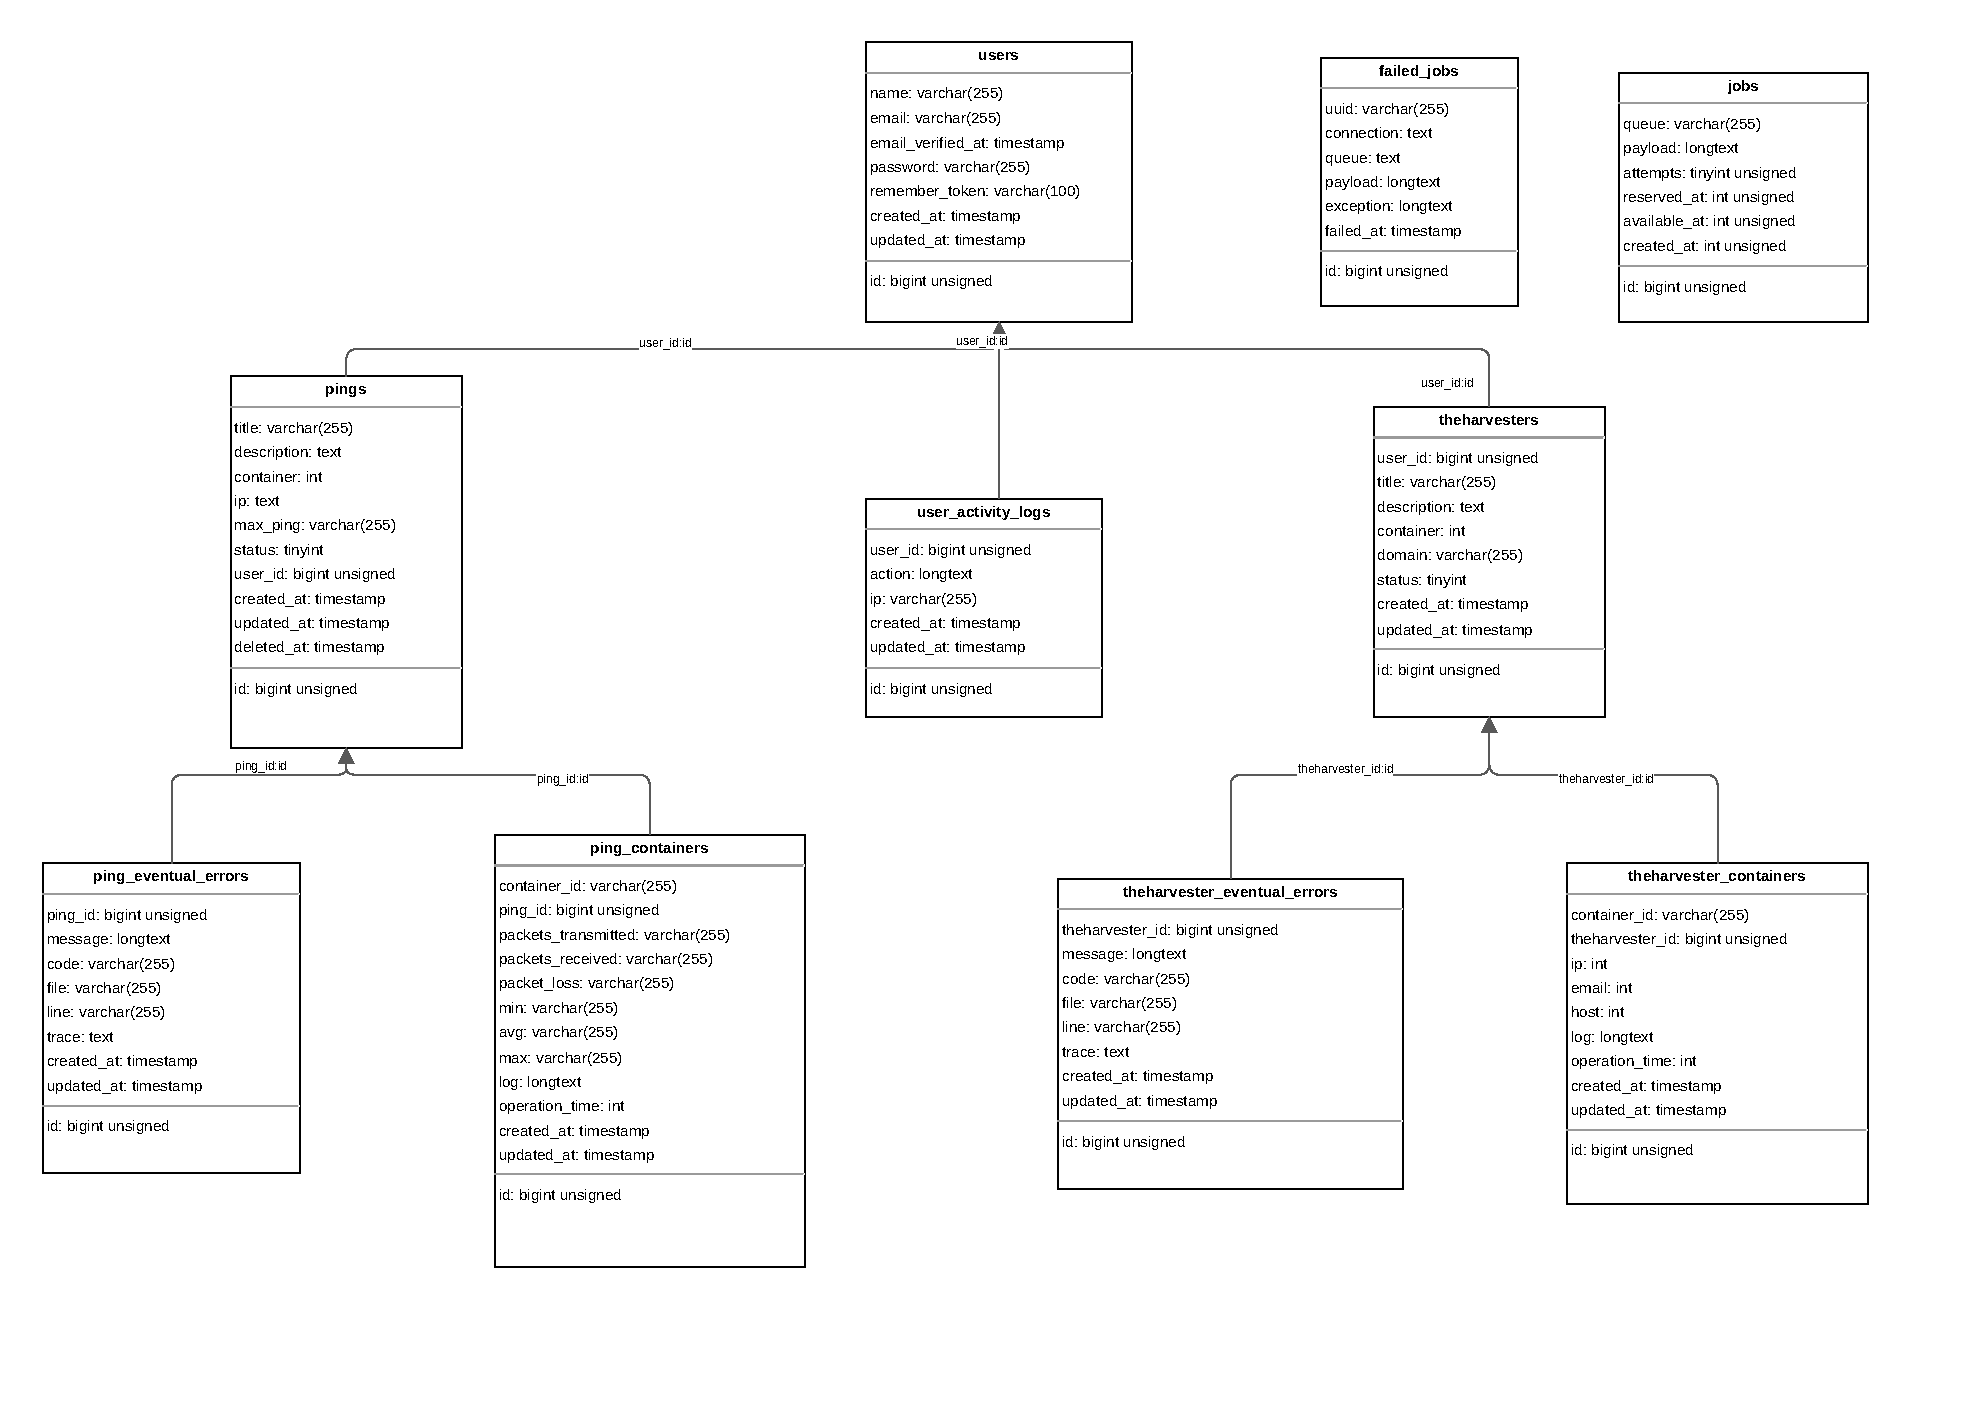
\includegraphics[width=\linewidth]{images/exported_from_idea.drawio.pdf}
  \caption{Veritabanı şeması}
  \label{fig:veritabani_diyagrami}
  \end{figure}
\subsection{Konteyner ile İlgili Temel Bilgiler}
Konteyner, bir uygulamanın çalışması için gereken tüm bağımlılıkları ve bileşenleri bir araya getiren ve bu bileşenlerin izole edilmiş bir ortamda çalışmasını sağlayan bir yazılım paketleme ve dağıtım teknolojisidir. Konteynerler, bir uygulamanın tüm çalışma zamanı bağımlılıklarını içeren taşınabilir bir ortam sunar ve böylece uygulamaların farklı platformlarda tutarlı bir şekilde çalışmasını sağlar \cite{domenici_bravo}.

Konteynerlerin avantajları şunlardır:
\begin{itemize}
  \item Taşınabilirlik: Konteynerler, uygulamaların bir ortamdan diğerine sorunsuz bir şekilde taşınmasını sağlar. Konteynerlerin bağımsız bir şekilde çalışabilmesi, farklı işletim sistemleri, bulut platformları veya dağıtım ortamları arasında sorun yaşamadan hareket etmelerini sağlar.
  \item İzolasyon: Konteynerler, uygulamaların birbirlerinden ve ana işletim sisteminden izole bir şekilde çalışmasını sağlar. Her konteyner, kendi dosya sistemine, ağ bağlantılarına ve kaynaklara sahiptir. Bu, uygulamaların birbirlerinin kaynaklarını etkilemeden güvenli bir şekilde çalışmasını sağlar.
  \item Hızlı Dağıtım: Konteynerler, hızlı ve tutarlı bir şekilde dağıtılabilir. Konteyner imajları, uygulamaların ve bağımlılıklarının bir araya getirildiği taşınabilir bir formattır. Bu imajlar hızlı bir şekilde oluşturulabilir, paylaşılabilir ve dağıtılabilir, böylece uygulamaların hızlı bir şekilde çalıştırılması ve güncellenmesi mümkün olur.
  \item Ölçeklenebilirlik: Konteynerler, uygulamaların kolayca ölçeklendirilmesini sağlar. Konteyner tabanlı bir uygulamanın birden fazla kopyası aynı anda çalıştırılabilir ve bir yük dengeleyici kullanılarak trafiğin bu kopyalar arasında dengeli bir şekilde dağıtılması sağlanabilir. Bu, yüksek talepler altında uygulamaların performansını artırır.
\end{itemize}

Konteynerlerin dezavantajları şunlardır:
\begin{itemize}
  \item Karmaşıklık: Konteyner teknolojileri, bazı kullanıcılar için karmaşık olabilir. Konteynerlerin oluşturulması, yönetimi ve yapılandırılması konusunda ek bilgi ve beceri gerektirebilir. Bu nedenle, konteyner teknolojilerini kullanmak isteyen kullanıcıların bu teknolojilere aşina olmaları ve gerektiğinde destek almaları önemlidir.
  \item Bellek ve İşlemci Kullanımı: Konteynerlerin izolasyonu sağlamak için ek sistem kaynaklarına ihtiyaçları olabilir. Konteynerler, her biri kendi işletim sistemleri gibi davranırken, her bir konteynerin bellek ve işlemci kullanımı ek yük getirebilir. Bu, sistem kaynaklarının daha dikkatli bir şekilde yönetilmesini gerektirebilir.
  \item Veri Yönetimi: Konteynerler, genellikle veri yönetimi konusunda bazı zorluklar sunabilir. Konteynerlerin geçici doğası ve izole edilmiş dosya sistemleri, verilerin nasıl depolanacağı, paylaşılacağı ve korunacağı konusunda bazı ek adımlar gerektirebilir. Bu, uygulama geliştiricilerinin veri yönetimi stratejilerini dikkate almalarını gerektirir.
\end{itemize}

Konteyner teknolojileri, uygulamaları hızlı bir şekilde dağıtmak, taşımak ve ölçeklendirmek için güçlü bir araçtır. Ancak, her çalışmanin ihtiyaçlarına ve altyapısına bağlı olarak avantajları ve dezavantajları dikkate almak önemlidir.

Çalışmanın ne olduğunu nasıl çalıştığı Bölüm \ref{sec:study}'te detaylıca anlatılmıştır.
\section{PROJE'NİN İŞLEYİŞİ}
\subsection{Arayüz Kısmı }
Bu projede  Arayüz  kısmı için işleyiş aşağıda belirtilmiştir.  \\
İsteklere uygun bir template bulundu ve template üzerinde projeye uygun hale getirildi. Gereksiz kısımlar temizlendi ve sağ menü bölümünde sırasıya Dashboard , görevler(Ping ,Theharvester), sistem logları ve Profil   bölümleri oluşturuldu. 

Proje ilk açıdığında kullanıcı login sayfası ile karşılaşacaktır.Kimlik bilgileri girlecektir.Doğrulama yaptıktan sonra diğer sayfalara erişebilecektir.Giriş yaptıktan sonra karşılaşacağı ilk sayfa  Kontrol Panelidir.Kontrol panelinde oluşabilecek işlemler yazılacak\\
Sağ kısımda menü bulunabilmektedir.Burda görevler kısmından istediği zaman görev oluşurup önceden oluşturulan o görevle ilgili işlemleri  de görebilir.Bir ping görevi  açıldığında oluşan konyetnerlar bu  konteynarların çıktıları , kayıp yzüdesi ,pingin maximum  geri dönüş süresi ,minimum geri dönüş süresi ve  ortalama milisaniye geri dönüş süresi bulunmaktadır .%Theharvester görevi de eklenecek
 Yine sağ menü kısmında sistem log kayıtları da görüntülenebilir .Bu log kayıtları altına ise kullanıcı Kim hangi görevi ne zaman çalıştırmış?, Görev kaç saniyede tamamlanmış?,Görev başarılı mı başarısız mı?,Oturum açma ve kapatma sorularının cevabını da kolaylıkla görüntüleyebilecektir.\\
Hesabım kısmından profil ile  ilgili düzenlemeler yapılabilir.

%arayüz fotoğrafları eklenecek 
\subsection{Arka paln işleyişi}

%ibrahim bu kısımda özet yazacak detaylandırılacak
 \subsection {Veritabanı kısmı Tabloların oluşturulması }
 
%\section{EK BÖLÜM}
%\section{ARAŞTIRMA BULGULARI VE TARTIŞMALAR} 
\section{SONUÇLAR VE ÖNERİLER}

Bu proje, konteyner teknolojilerinin yaygınlaşmasıyla birlikte ortaya çıkan karmaşıklığı azaltmak amacıyla geliştirilmiştir. Konteyner kullanımını kolaylaştırmayı hedefleyen bu projede, konteyner oluşturma, çalıştırma ve sonuçları başarıyla gerçekleştirilmektedir. 

Projenin başarılı sonuçları aşağıdaki şekillerde değerlendirilebilir:
\begin{itemize}
    \item Konteyner İşlemleri: Proje, Docker Engine API ile entegre olarak konteyner oluşturma, çalıştırma, durdurma ve silme gibi işlemleri başarılı bir şekilde gerçekleştirmektedir. Bu sayede kullanıcılar, Docker konteynerlerini kolaylıkla yönetebilmektedir.
    \item Çalışma Performansı: Projenin uygulama performansı, Guzzle kütüphanesinin etkili kullanımı ve Docker Engine API'nin sağladığı hızlı yanıtlar sayesinde yüksek seviyede tutulmaktadır. Bu da kullanıcı deneyimini olumlu yönde etkilemektedir.
    \item Theharvester Servisi: Proje, servislerin eklenmesini desteklemektedir. Örnek olarak Theharvester servisi geliştirilmiş ve başarıyla projeye entegre edilmiştir. Bu sayede kullanıcılar, projelerine farklı servisleri ekleyerek genişletme imkanına sahip olmaktadır.
\end{itemize}




\subsection*{Öneriler}
\begin{itemize}
    \item Kullanıcı Arayüzü Geliştirme: Gelecekte, web tabanlı bir kullanıcı arayüzü oluşturulabilir. Bu arayüz sayesinde kullanıcılar, konteyner oluşturma, silme, güncelleme ve sonuçları inceleme gibi işlemleri görsel bir şekilde gerçekleştirebilir. Bu, kullanım kolaylığı sağlayacak ve projenin kullanıcı tabanını genişletecektir.
    \item Hata Yönetimi ve Güncelleme: Proje, hataların ve istisnaların yönetimini etkin bir şekilde gerçekleştirmektedir. Gelecekte, kullanıcı geri bildirimleri ve testlerle projenin daha da güçlendirilmesi ve hata sayısının en aza indirgenmesi sağlanabilir. Ayrıca, Docker Engine API'nin güncellemelerini takip etmek ve projeyi güncel tutmak da önemlidir.
    \item Dokümantasyon ve Destek: Projeye ilişkin kapsamlı bir dokümantasyon oluşturmak, kullanıcıların projeyi daha iyi anlamalarını ve kullanmalarını sağlayacaktır. Ayrıca, kullanıcıların karşılaştıkları sorunlar için destek sağlamak da önemlidir. Sorunların çözümüne yönelik bir destek kanalı veya topluluk oluşturmak, kullanıcı memnuniyetini artıracaktır.
    \item Genişletilebilirlik: Projeye ekstra servisler eklemek için Laravel paketlerinin geliştirilmesi teşvik edilmelidir. Geliştiricilere açık API ve belgeleme sağlanarak, yeni servislerin kolayca entegre edilebilmesi ve projenin kullanım alanının genişlemesi sağlanabilir.
\end{itemize}

Sonuç olarak, bu proje konteyner teknolojilerinin karmaşıklığını azaltarak kullanım kolaylığı sağlamak amacıyla geliştirilmiştir. Başarılı sonuçları ve önerilerle birlikte, projenin gelecekteki gelişim potansiyeli ve kullanıcı memnuniyetini artırma imkanı vardır.
\section{EKLER}


% kaynak başlığını tanımlar
\renewcommand{\refname}{KAYNAKLAR}

\addcontentsline{toc}{section}{KAYNAKLAR}
\begin{thebibliography}{99} %kaynak ortamı 
\bibitem{k1}\url{https://store.steampowered.com/app/375820/Human_Resource_Machine/} [Ziyaret Tarihi: 30 Mayıs 2022]
\bibitem{k2}\url{https://tr.wikipedia.org/wiki/GitHub} [Ziyaret Tarihi: 6 Nisan 2022]
\bibitem{k3}\url{https://sungraphica.itch.io/sci-fi-game-ui-collection-free-version} [Ziyaret Tarihi: 6 Nisan 2022] 
 [Ziyaret Tarihi: 6 Nisan 2022] 
\end{thebibliography}
\centerline{\textbf{ÖZGEÇMİŞ}}
\addcontentsline{toc}{section}{ÖZGEÇMİŞ}
\begin{table}[H]
{
\renewcommand{\arraystretch}{1.5}
\begin{tabular}{l@{\bf :}l}
\multicolumn{2}{l}{\underline{\bf KİŞİSEL BELGELER}}\cr
\textbf{Adı Soyadı}& \;      \cr 
\textbf{Uyruğu}&\; T.C. \cr
\textbf{Doğum Yeri ve Tarihi}&\;      \cr
\textbf{Adres}&\;      \cr
\multicolumn{1}{l}{}&      \cr
\textbf{Telefon}&\;   \cr
\textbf{E-mail}&\;     \cr
\multicolumn{1}{l}{}&\cr
\multicolumn{2}{l}{\underline{\bf EĞİTİM DURUMU}}\cr
\textbf{Lisans Öğrenimi}&\; BŞEÜ Bilgisayar Mühendisliği Bölümü\cr
\textbf{Bitirme Yılı}&\;     \cr
\textbf{Lise}& \;     \cr
\multicolumn{1}{l}{}&\cr
\multicolumn{2}{l}{\underline{\bf İŞ DENEYİMLERİ}}\cr
\textbf{Yıl}&\;      \cr
\textbf{Kurum}& \;     \cr
\textbf{Stajlar}&\;      \cr
\multicolumn{1}{l}{}&\cr
\multicolumn{2}{l}{\underline{\bf İLGİ ALANLARI:}} \cr
\multicolumn{1}{l}{ }&  \cr
\multicolumn{1}{l}{}&  \cr

\multicolumn{2}{l}{\underline{\bf YABANCI DİLLER:}} \cr
\multicolumn{1}{l}{ }&\cr
\multicolumn{1}{l}{}&  \cr

\multicolumn{2}{l}{\underline{\bf BELİRTMEK İSTEDİÐİNİZ DİĞER ÖZELLİKLER:}}
\end{tabular}}
\end{table}

\end{document}
%%%%%%%%%%%%%%%%%%%%%%%%%%%BİTTİ%%%%%%%%%%%%%%%%%%%%%%%%%%%%%%%%%%% 